\section{Syntax trees and canonical derivations}

\begin{definition}[\textit{Syntax tree}]
    A syntax tree is a directed, ordered graph devoid of cycles.
    In this graph, nodes are arranged from left to right, and for any pair of nodes, there exists only one connecting path.
\end{definition}
Key features of a syntax tree include:
\begin{itemize}
    \item Visualization of the derivation process.
    \item Relationships such as parent-child, descendants, root node, and leaf or terminal nodes.
    \item The degree of a node is determined by the number of its children.
    \item The root node represents the axiom $S$.
    \item The tree's frontier contains the generated phrase.
\end{itemize}
Various subtrees can be defined from a syntax tree by selecting a node $N$ as the new root.
\begin{example}
    The sentence $i+i*i$ can be represented in a syntax tree, following the rules for sum and product, as depicted below:
    \begin{figure}[H]
        \centering
        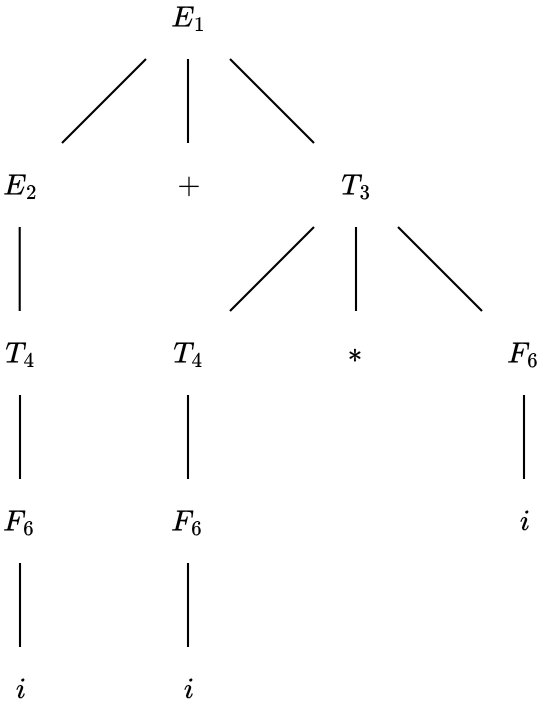
\includegraphics[width=0.25\linewidth]{images/syntree.png}
    \end{figure}
    It can also be expressed in a linear form:
    \[[[[[i]_F]_T]_E+[[[i]_F]_T*[i]_F]_T]_E\]
\end{example}

\paragraph*{Ambiguity}
Right derivation (expanding the rightmost non-terminal at each step) and left derivation (expanding the leftmost non-terminal at each step) are possible.
For a given syntax tree, there exists a unique right derivation and a unique left derivation corresponding to that tree.
Both right and left derivations are useful for defining parsing algorithms.
The ambiguity of a grammar is determined by whether a given sentence has a unique syntax tree.

\paragraph*{Construction}
To construct a correct syntax tree, it is important to consider:
\begin{itemize}
    \item Deriving nonterminals for low-precedence operators first.
    \item Deriving nonterminals for high-precedence operators later.
\end{itemize}
\begin{definition}[\textit{Skeleton tree}]
    A skeleton tree is a syntax tree that preserves only the frontier and structure.
\end{definition}
\begin{definition}[\textit{Condensed skeleton tree}]
    A condensed skeleton tree is a syntax tree in which internal nodes on non-branching paths are merged.
\end{definition}
\begin{example}
    The syntax tree from the previous example can be transformed into a skeleton tree:
    \begin{figure}[H]
        \centering
        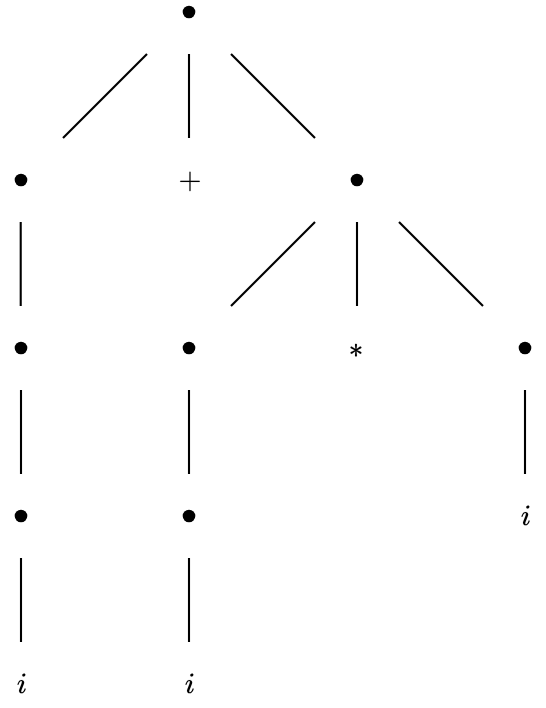
\includegraphics[width=0.25\linewidth]{images/syntree1.png}
    \end{figure}
    With the corresponding linear form:
    \[[[[[i]]]+[[[i]]*[i]]]\]
    It can also be transformed into a condensed skeleton tree:
    \begin{figure}[H]
        \centering
        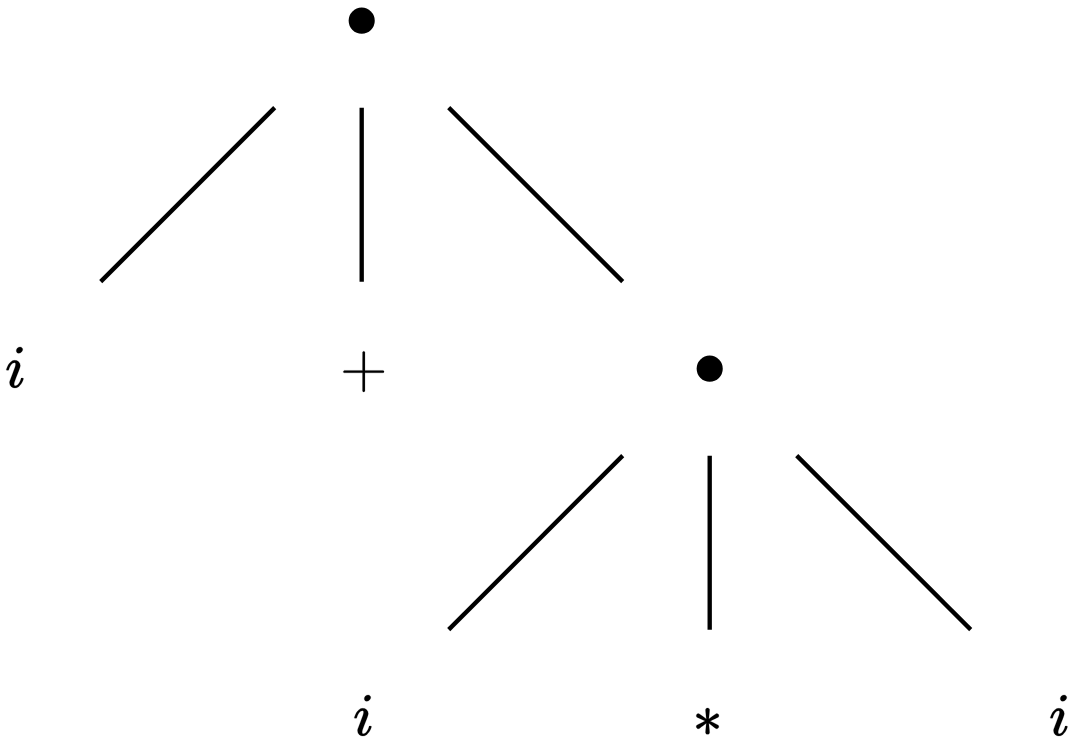
\includegraphics[width=0.25\linewidth]{images/syntree2.png}
    \end{figure}
    With the corresponding linear form:
    \[[[i]+[[i]*[i]]]\]
\end{example}